% ********** Rozdział 4 **********
\chapter{Prezentacja warstwy użytkowej projektu}

Aplikacja jest interaktywną grą RPG, w której gracze mogą eksplorować różne lokacje, 
walczyć z przeciwnikami oraz rozwijać swoje postacie. Gra oferuje różnorodne mechaniki, takie jak system walki, tworzenia przedmiotów, wykonywania misji oraz interakcje z NPC. 
Użytkownicy mogą również zarządzać swoim ekwipunkiem oraz brać udział w zadaniach.

\section{Prezentacja}
W tej sekcji przedstawiono zrzuty ekranu i opisy ilustrujących kluczowe interfejsy i funkcjonalności aplikacji.
\subsection{Menu główne}
\begin{itemize}
    \item Na rysunku 4.1 przedstawiono głowne menu aplikacji, które ukazuje się po włączeniu jej. 
    Aplikacja pozwala na rozpoczęcie nowej gry, załadowanie lub usunięcie istniejącego zapisu gry, zmianę języka, lub wyjście z gry.
        \begin{figure}[H]
            \centering
            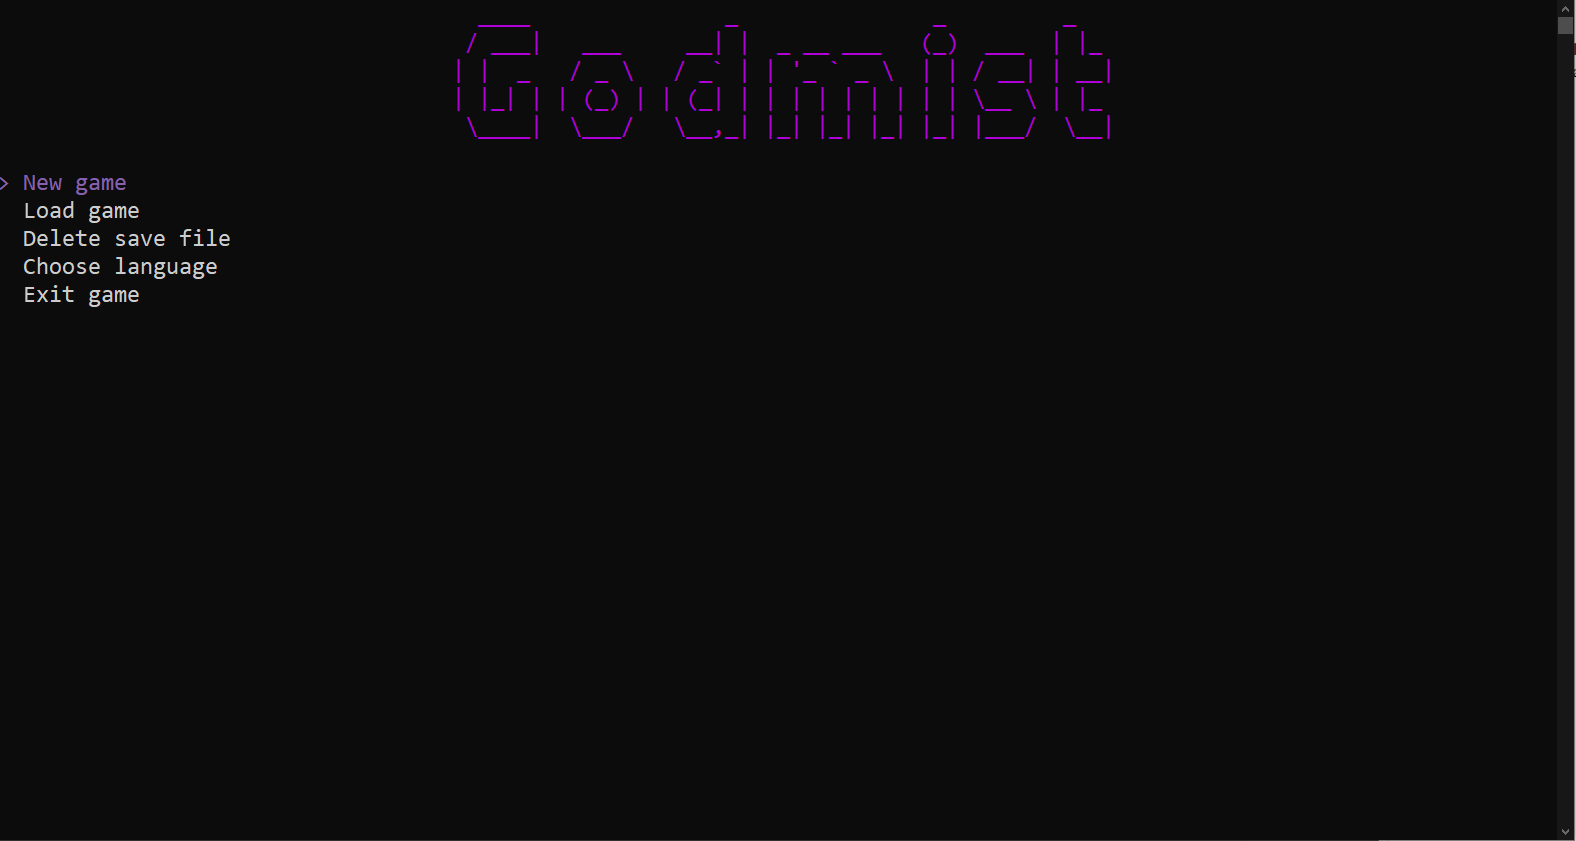
\includegraphics[width=0.8\textwidth]{figures/warstwa_uzytkowa/menu_glowne_1.png}
            \caption{Menu główne, opcje początkowe}
            \label{fig:main_menu_1}
        \end{figure}
        \item Na rysunku 4.2 przedstawiono wybór języka dostępny z głównego menu. Po wybraniu języka aplikacja wraca do początkowego ekranu. 
        (język zmieniono na polski)
            \begin{figure}[H]
                \centering
                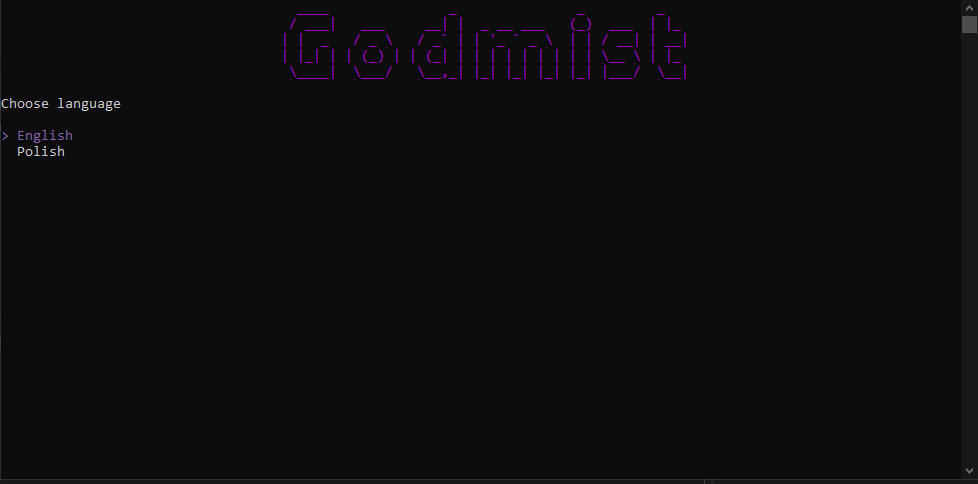
\includegraphics[width=0.8\textwidth]{figures/warstwa_uzytkowa/menu_glowne_2.png}
                \caption{Menu główne, wybór języka}
                \label{fig:main_menu_2}
            \end{figure}
        \item Na rysunku 4.3 przedstawiono wybór poziomu trudności, dostępny po rozpoczęciu nowej gry.
            \begin{figure}[H]
                \centering
                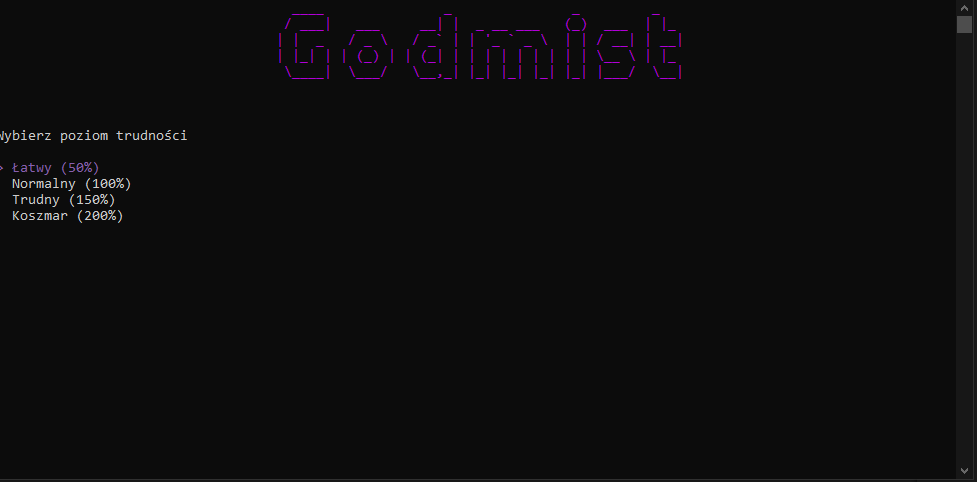
\includegraphics[width=0.8\textwidth]{figures/warstwa_uzytkowa/menu_glowne_3.png}
                \caption{Menu główne, wybór poziomu trudności}
                \label{fig:main_menu_3}
            \end{figure}
        \item Po wybraniu poziomu trudności, gra przedstawia wprowadzenie oraz pozwala na wybranie klasy postaci. 
        Na rysunku 4.4 znajduje się wybór klasy postaci.
            \begin{figure}[H]
                \centering
                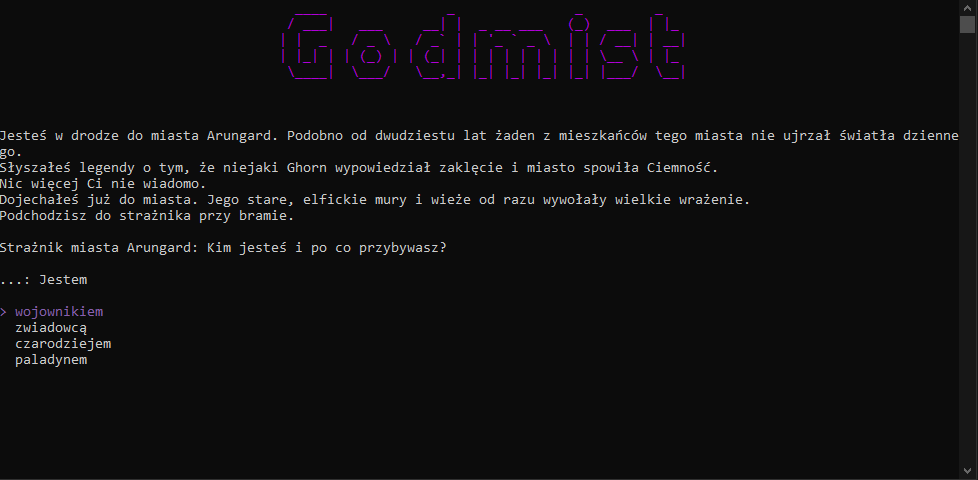
\includegraphics[width=0.8\textwidth]{figures/warstwa_uzytkowa/menu_glowne_4.png}
                \caption{Menu główne, wybór klasy postaci}
                \label{fig:main_menu_4}
            \end{figure}
        \item Po wybraniu klasy postaci, gra pozwala na wybranie nazwy postaci. 
        Aplikacja zabezpieczona jest przed wpisaniem pustej nazwy (wciśniecie klawisza Enter nie przenosi dalej), 
        lub zbyt długiej (otrzymujemy informację zwrotną). Na rysunku 4.5 przedstawiono wybór nazwy postaci.
            \begin{figure}[H]
                \centering
                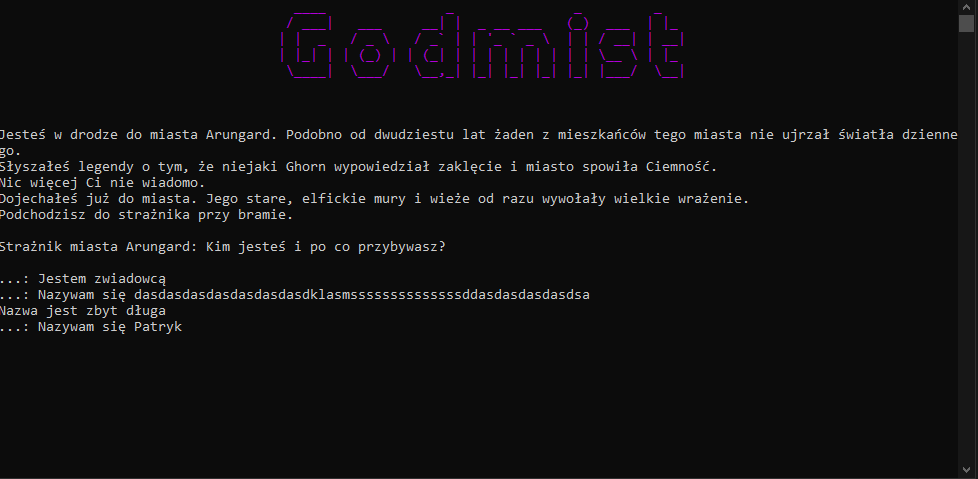
\includegraphics[width=0.8\textwidth]{figures/warstwa_uzytkowa/menu_glowne_5.png}
                \caption{Menu główne, wybór nazwy}
                \label{fig:main_menu_5}
            \end{figure}
\end{itemize}
\subsection{Miasto}
\begin{itemize}
        \item Po wybraniu nazwy, gracz przenoszony jest do miasta. Otrzymuje wiele opcji takich jak wyruszenie na wyprawę do lochu, 
        rozmawianie z NPC, otwarcie dziennika zadań, ekwipunku, włączenie okna postaci, zapis gry, lub powrót do menu. 
        Na rysunku 4.6 przedstawiono ekran główny miasta.
            \begin{figure}[H]
                \centering
                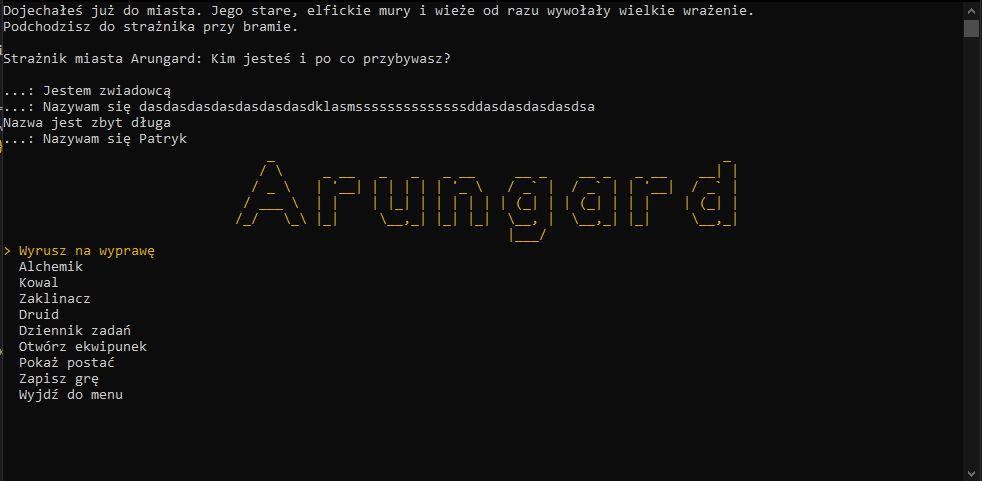
\includegraphics[width=0.8\textwidth]{figures/warstwa_uzytkowa/miasto_1.png}
                \caption{Miasto, ekran główny}
                \label{fig:city_1}
            \end{figure}
        \item Jeśli użytkownik wybierze opcję `Zapisz grę', zostaje zapytany o podanie nazwy pliku zapisu, który chce utworzyć. 
        Tutaj również występuje zabezpieczenie przed pustą i zbyt długą nazwą. Po wpisaniu nazwy plik zapisu tworzy się, a 
        gracz ponownie otrzymuje ekran głowny miasta. Na rysunku 4.7 przedstawiono proces zapisu gry.
            \begin{figure}[H]
                \centering
                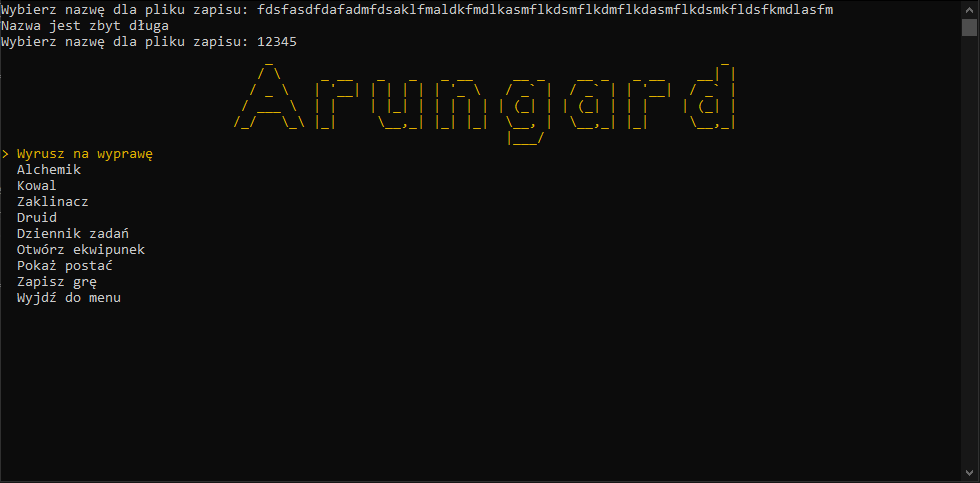
\includegraphics[width=0.8\textwidth]{figures/warstwa_uzytkowa/miasto_2.png}
                \caption{Miasto, zapis gry}
                \label{fig:city_2}
            \end{figure}
        \item Jeśli użytkownik wybierze opcję `Pokaż postać', wyświetlone zostają informacje o statystykach i wyposażeniu postaci.
        Po naciśnięciu dowolnego przycisku na klawiaturze, gracz ponownie otrzymuje ekran główny miasta. Na rysunku 4.8 przedstawiono ekran postaci.
            \begin{figure}[H]
                \centering
                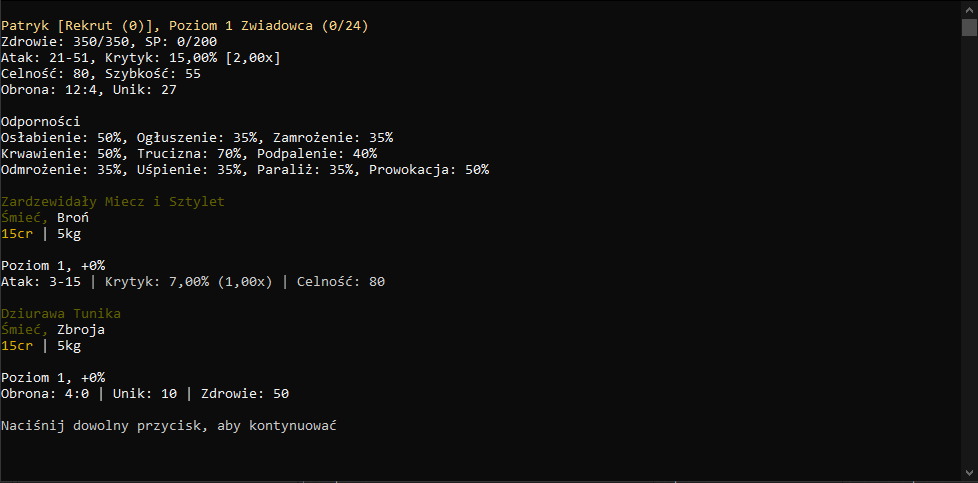
\includegraphics[width=0.8\textwidth]{figures/warstwa_uzytkowa/miasto_3.png}
                \caption{Ekran postaci}
                \label{fig:city_3}
            \end{figure}
\end{itemize}
\subsection{Postacie niezależne}
\begin{itemize}
    \item Po wybraniu opcji `Alchemik', `Kowal' lub `Zaklinacz', gracz zostanie przeniesiony do rozmowy z odpowiednim NPC. Stąd może
    wykonać jedną z dostępnych akcji, takich jak wejście do sklepu, czy wyleczenie ran. Na rysunku 4.9 przedstawiono okno alchemika.
        \begin{figure}[H]
            \centering
            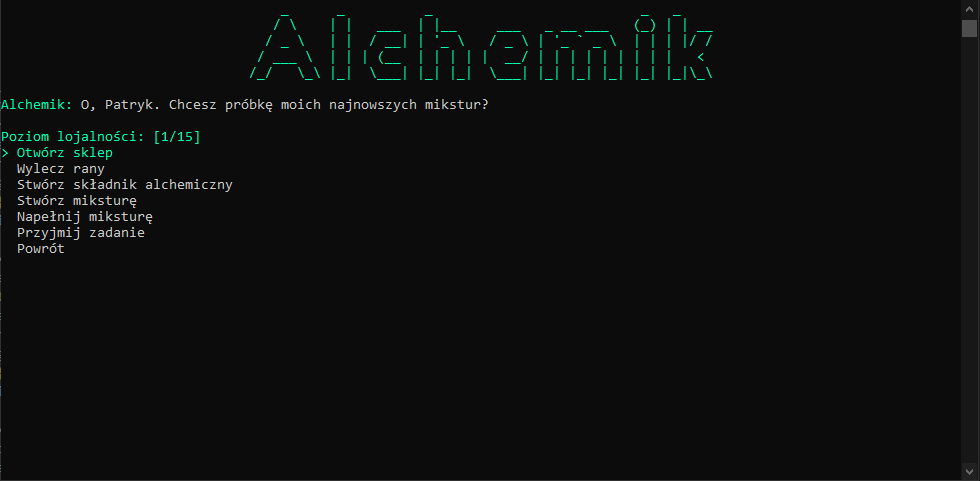
\includegraphics[width=0.8\textwidth]{figures/warstwa_uzytkowa/npc_1.png}
            \caption{Ekran NPC}
            \label{fig:npc_1}
        \end{figure}
    \item W przypadku, gdy użytkownik wybierze `Otwórz sklep', otworzy się okno przedstawiające listę przedmiotów posiadanych przez postać niezależną.
    Tutaj, ma tak jak w ekwipunku opcje zbadania wybranego przedmiotu. Może również kupować przedmioty od NPC, 
    lub sprzedawać przedmioty ze swojego ekwipunku. Na rysunkach 4.10 i 4.11 przedstawiono menu sklepu.
        \begin{figure}[H]
            \centering
            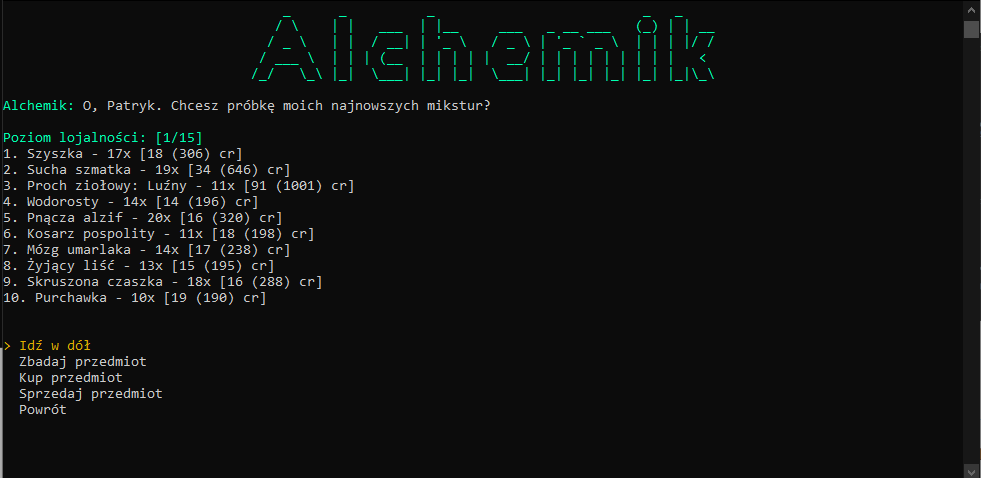
\includegraphics[width=0.8\textwidth]{figures/warstwa_uzytkowa/npc_2.png}
            \caption{Menu sklepu NPC, widok początkowy}
            \label{fig:npc_2}
        \end{figure}
        \begin{figure}[H]
            \centering
            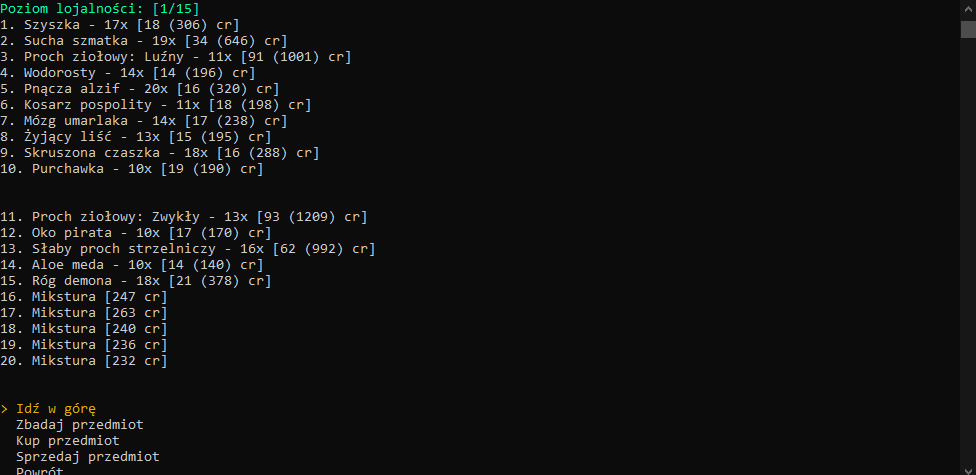
\includegraphics[width=0.8\textwidth]{figures/warstwa_uzytkowa/npc_3.png}
            \caption{Menu sklepu NPC, po wybraniu `Idź w dół'}
            \label{fig:npc_3}
        \end{figure}
    \item Po wybraniu opcji `Zbadaj przedmiot', ukazuje się się pole wyboru przedmiotu z ekwipunku alchemika. 
    Po wybraniu z listy, przedstawione zostają szczegóły badanego przedmiotu. Na rysunkach 4.12 i 4.13 przedstawiono proces badania przedmiotu.
        \begin{figure}[H]
            \centering
            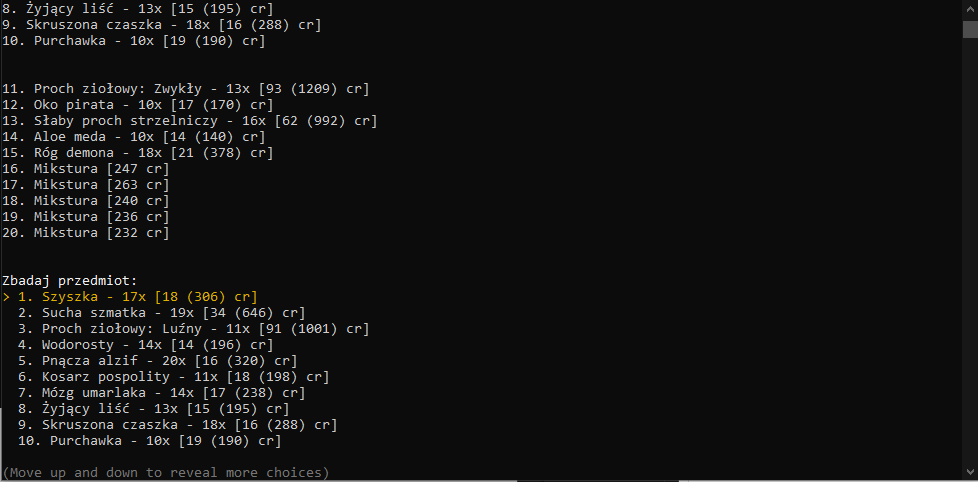
\includegraphics[width=0.8\textwidth]{figures/warstwa_uzytkowa/npc_4.png}
            \caption{Menu sklepu NPC, badanie przedmiotu, wybór}
            \label{fig:npc_4}
        \end{figure}
        \begin{figure}[H]
            \centering
            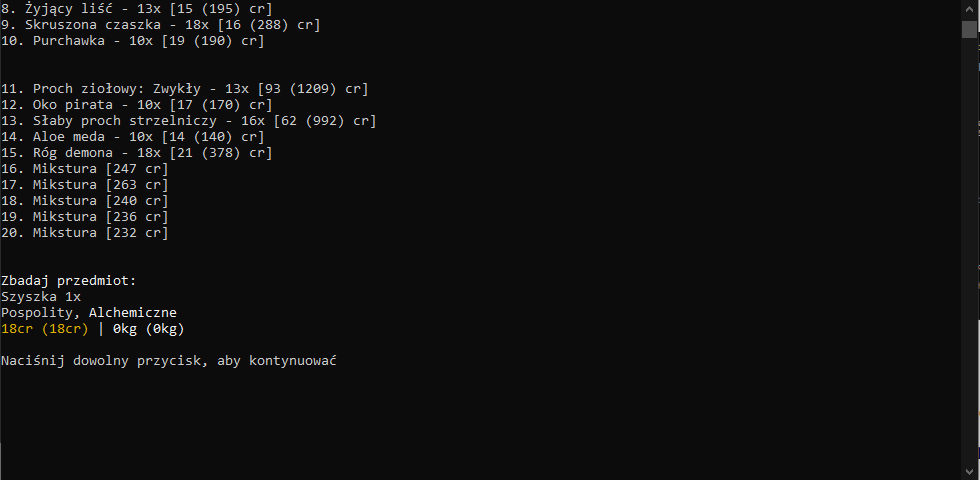
\includegraphics[width=0.8\textwidth]{figures/warstwa_uzytkowa/npc_5.png}
            \caption{Menu sklepu NPC, badanie przedmiotu, rezultat}
            \label{fig:npc_5}
        \end{figure}
    \item Po wybraniu opcji `Kup przedmiot`, użytkownik otrzymuje identyczne okno wyboru. 
    Po jego dokonaniu i potwierdzeniu, że chce kupić przedmiot, otrzymuje go i traci złoto. Kupowanie przedmiotu przedstawiono na rysunku 4.14
        \begin{figure}[H]
            \centering
            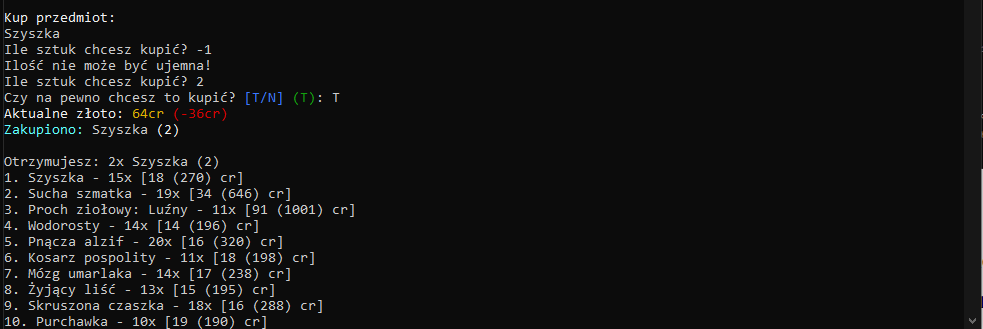
\includegraphics[width=0.8\textwidth]{figures/warstwa_uzytkowa/npc_6.png}
            \caption{Menu sklepu NPC, kupno przedmiotu}
            \label{fig:npc_6}
        \end{figure}
    \item Po wybraniu opcji `Sprzedaj przedmiot`, użytkownik może wybrać przedmiot ze swojego ekwipunku
    Po wybraniu przedmiotu i potwierdzeniu, że chce sprzedać przedmiot, traci go i zyskuje złoto.
    Na rysunkach 4.15 i 4.16 przedstawiono proces sprzedaży przedmiotu
        \begin{figure}[H]
            \centering
            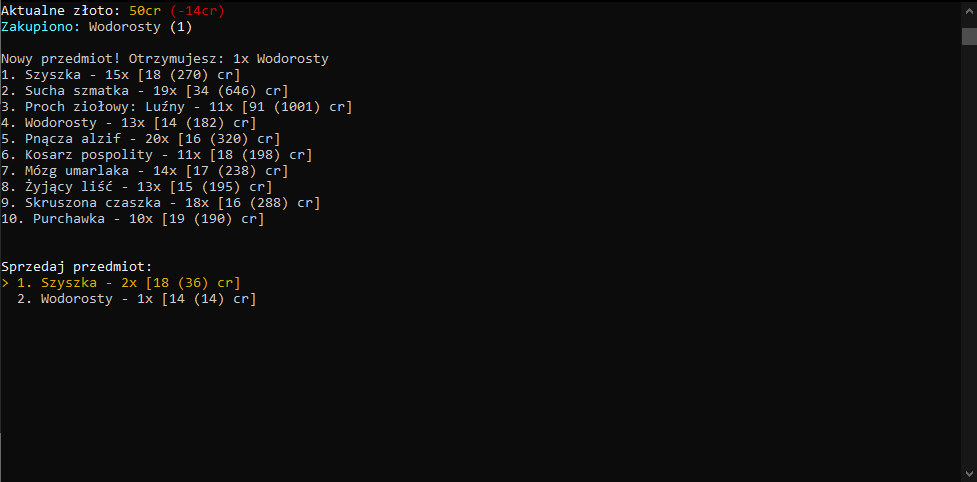
\includegraphics[width=0.8\textwidth]{figures/warstwa_uzytkowa/npc_7.png}
            \caption{Menu sklepu NPC, sprzedaż przedmiotu, wybór}
            \label{fig:npc_7}
        \end{figure}
        \begin{figure}[H]
            \centering
            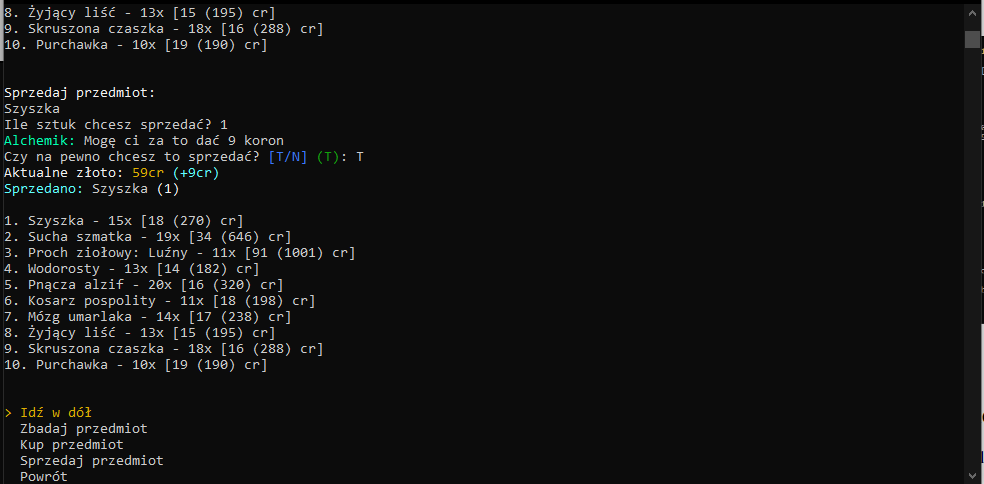
\includegraphics[width=0.8\textwidth]{figures/warstwa_uzytkowa/npc_9.png}
            \caption{Menu sklepu NPC, sprzedaż przedmiotu, rezultat}
            \label{fig:npc_9}
        \end{figure}
    \item Jeśli NPC posiada zadanie do zaoferowania, użytkownik może wybrać `Przyjmij zadanie'. Otrzymuje następnie wybór z dostępnych zadań u NPC.
    Po dokonaniu wyboru i potwierdzeniu go, zadanie zostaje zaakceptowane. Na rysunkach 4.17 i 4.18 przedstawiono akceptowanie zadania od NPC.
        \begin{figure}[H]
            \centering
            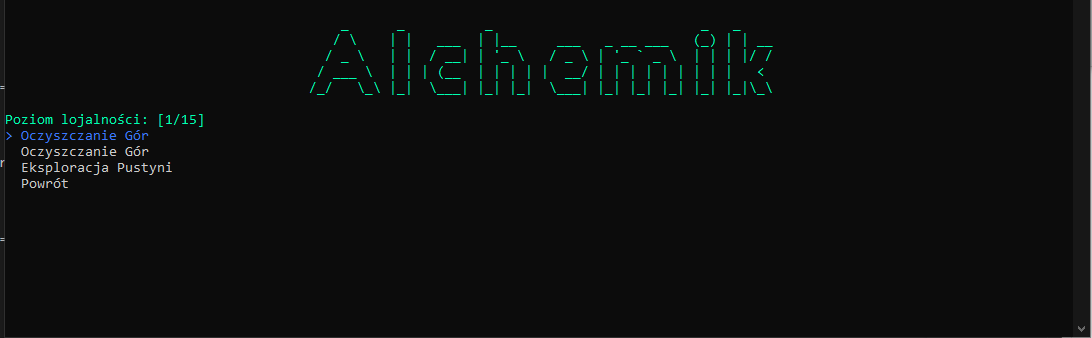
\includegraphics[width=0.8\textwidth]{figures/warstwa_uzytkowa/npc_10.png}
            \caption{Ekran NPC, wybór zadania}
            \label{fig:npc_10}
        \end{figure}
        \begin{figure}[H]
            \centering
            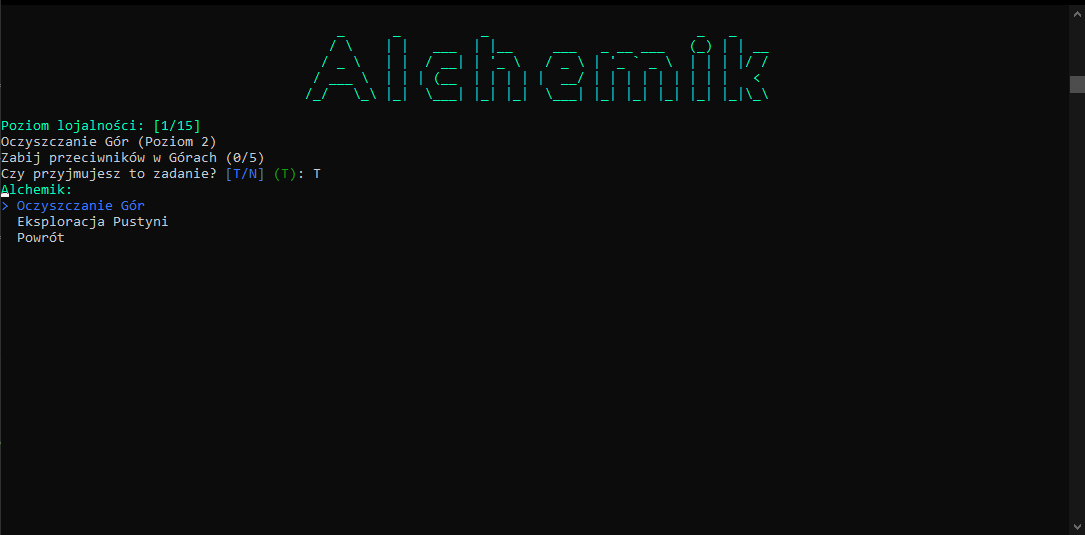
\includegraphics[width=0.8\textwidth]{figures/warstwa_uzytkowa/npc_11.png}
            \caption{Ekran NPC, zaakceptowane zadanie}
            \label{fig:npc_11}
        \end{figure}
\end{itemize}
\subsection{Ekwipunek}
\begin{itemize}
        \item Jeśli użytkownik wybierze opcję "Otwórz ekwipunek" w mieście lub w lochu, wyświetlone zostają informacje o ekwipunku i opcje zarządzania nim.
        Na rysunku 4.19 przedstawiono okno ekwipunku.
            \begin{figure}[H]
                \centering
                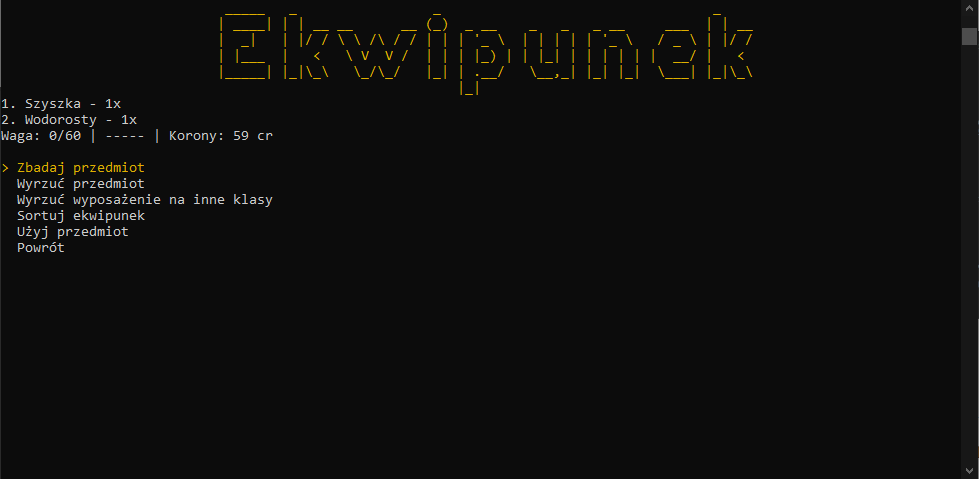
\includegraphics[width=0.8\textwidth]{figures/warstwa_uzytkowa/ekwipunek_1.png}
                \caption{Ekran ekwipunku}
                \label{fig:inventory_1}
            \end{figure}
        \item Gracz może zbadać dowolny przedmiot z ekwipunku, wyświetlone zostaną wtedy szczegóły tego konkretnego przedmiotu, 
        lub jeśli przedmiot spełnia własność `Stackable', to stosu przedmiotu. Na rysunkach 4.20 i 4.21 przedstawiono kolejne kroki badania przedmiotu.
            \begin{figure}[H]
                \centering
                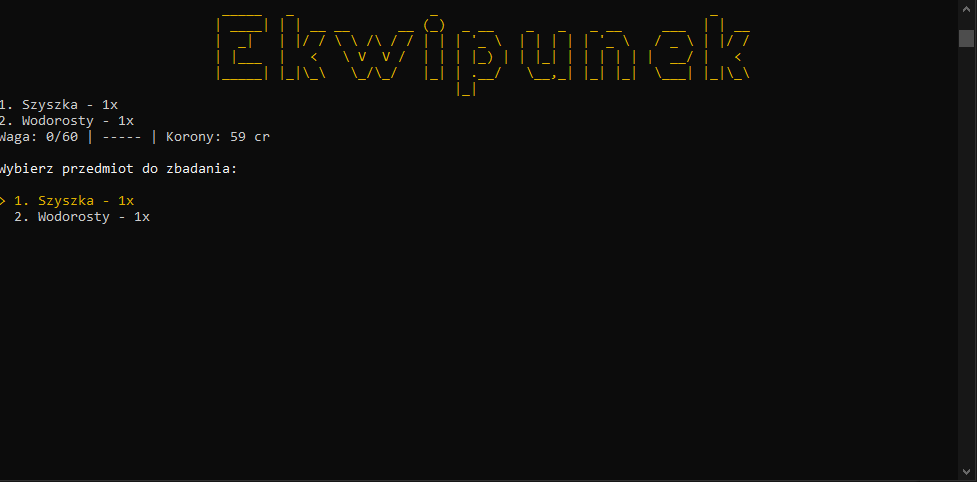
\includegraphics[width=0.8\textwidth]{figures/warstwa_uzytkowa/ekwipunek_2.png}
                \caption{Ekran ekwipunku. Badanie przedmiotu, wybór.}
                \label{fig:inventory_2}
            \end{figure}
            \begin{figure}[H]
                \centering
                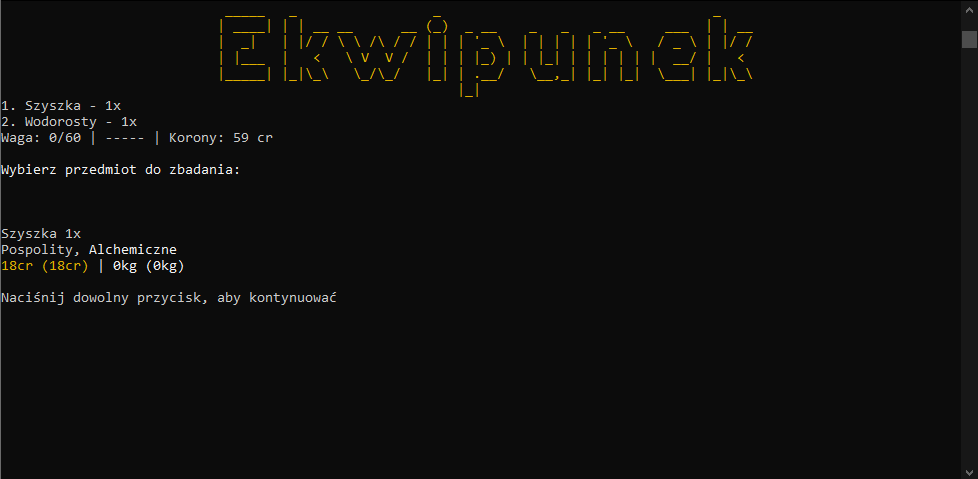
\includegraphics[width=0.8\textwidth]{figures/warstwa_uzytkowa/ekwipunek_3.png}
                \caption{Ekran ekwipunku. Badanie przedmiotu, rezultat.}
                \label{fig:inventory_3}
            \end{figure}
        \item Gracz może wyrzucić dowolny przedmiot z ekwipunku, zostanie on wtedy po potwierdzeniu usunięty z ekwipunku.
        Na rysunku 4.22 przedstawiono wyrzucanie przedmiotu
            \begin{figure}[H]
                \centering
                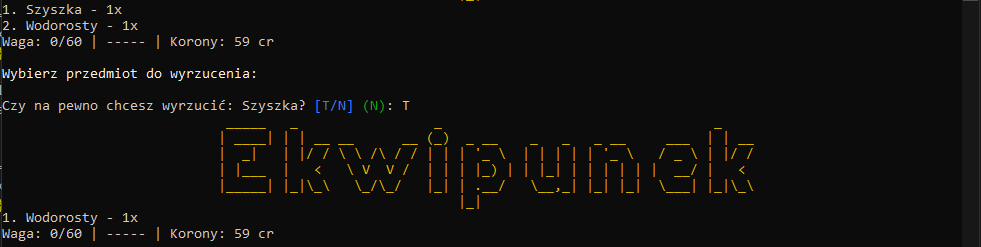
\includegraphics[width=0.8\textwidth]{figures/warstwa_uzytkowa/ekwipunek_4.png}
                \caption{Ekran ekwipunku, wyrzucanie przedmiotu.}
                \label{fig:inventory_4}
            \end{figure}
        \item Po kliknięciu `Wyrzuć wyposażenie na inne klasy', po potwierdzeniu zostaną usunięte wszystkie elementy wyposażenia 
        (bronie i pancerze), które nie mogą zostać użyte przez klasę postaci gracza.
        \item Po kliknieciu `Sortuj ekwipunek', ukazane zostaną możliwości sortowania ekwipunku na różne sposoby. 
        Po wybraniu opcji, ekwipunek zostanie posortowany według wybranego kryterium. Na rysunkach 4.23 i 4.24 przedstawiono sortowanie ekwipunku alfabetycznie.
            \begin{figure}[H]
                \centering
                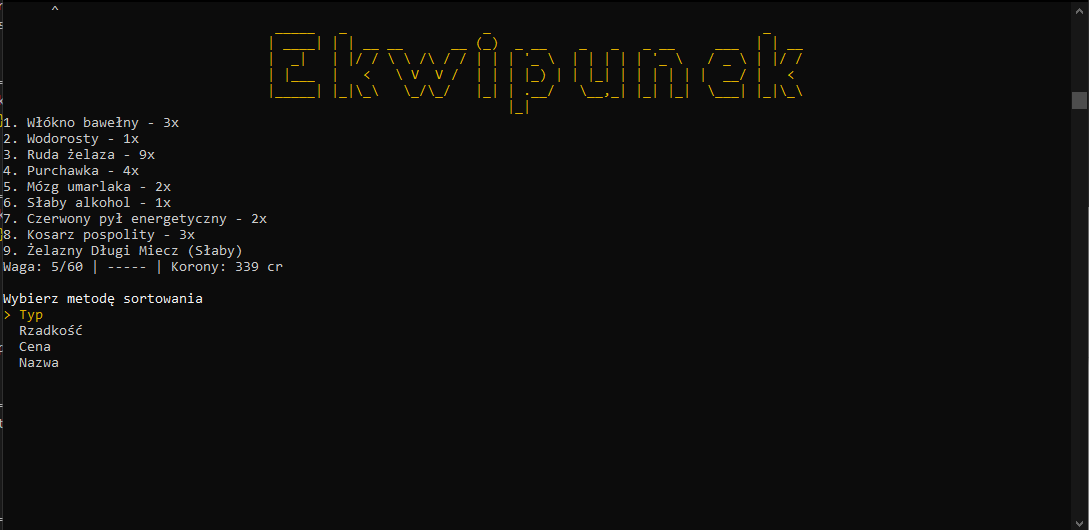
\includegraphics[width=0.8\textwidth]{figures/warstwa_uzytkowa/ekwipunek_5.png}
                \caption{Ekran ekwipunku, sortowanie ekwipunku, wybór metody.}
                \label{fig:inventory_5}
            \end{figure}
            \begin{figure}[H]
                \centering
                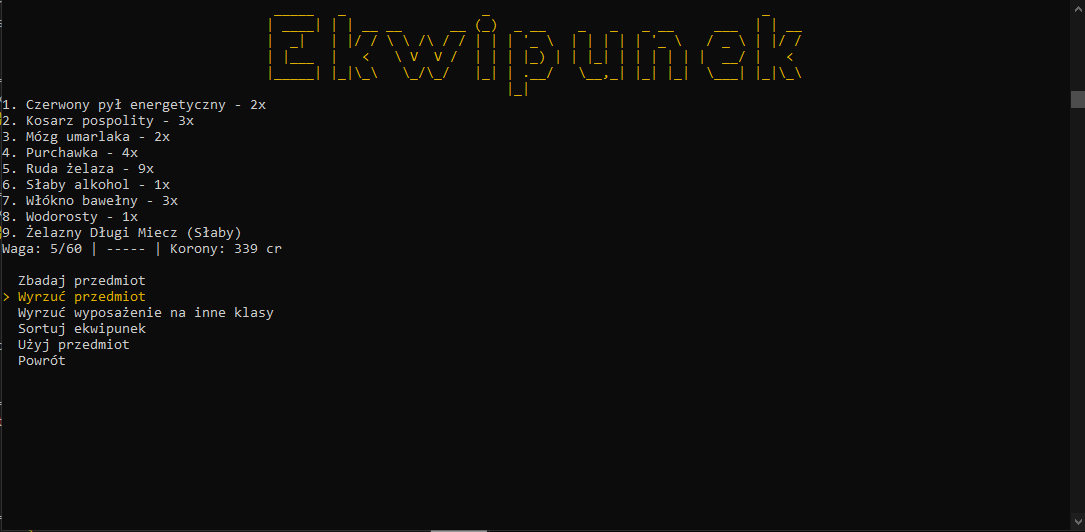
\includegraphics[width=0.8\textwidth]{figures/warstwa_uzytkowa/ekwipunek_6.png}
                \caption{Ekran ekwipunku, sortowanie ekwipunku, rezultat.}
                \label{fig:inventory_6}
            \end{figure}
        \item W przypadku wybrania opcji `Użyj przedmiot', użytkownik może wybrać przedmiot do użycia. 
        Jeśli będzie to przedmiot, który dziedziczy po \texttt{IUsable}, to wykona się akcja odpowiednia dla tego przedmiotu (użyta mikstura, wyposażona broń, itp.).
\end{itemize}
\subsection{Lochy}
\begin{itemize}
        \item Poprzez opcję `Wyrusz na wyprawę' w mieście, istnieje możliwość wygenerowania i wejścia do instancji lochu.
        Na rysunku 4.25 przedstawiono proces wejścia do lochu Katakumb na poziomie 1. Na rysunku 4.26 przedstawiono widok startowy lochu.
            \begin{figure}[H]
                \centering
                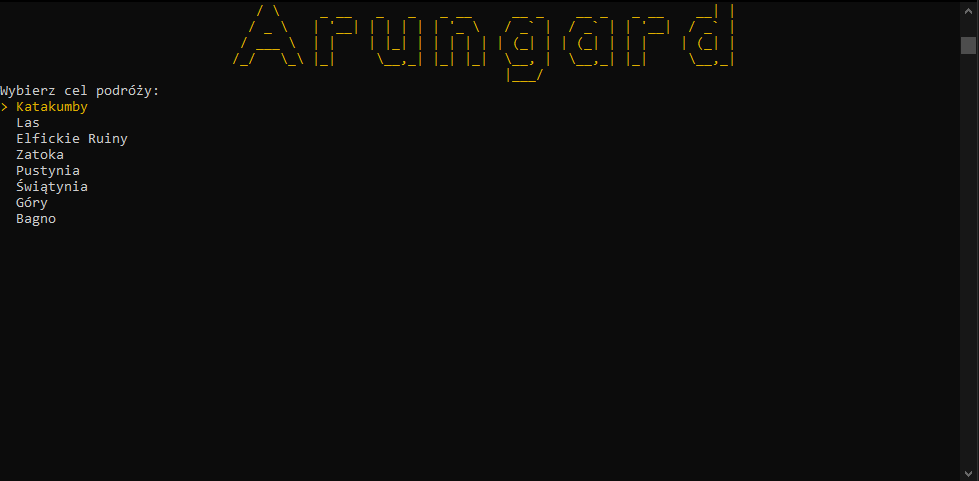
\includegraphics[width=0.8\textwidth]{figures/warstwa_uzytkowa/lochy_1.png}
                \caption{Lochy, wybór typu lochu}
                \label{fig:dungeons_1}
            \end{figure}
            \begin{figure}[H]
                \centering
                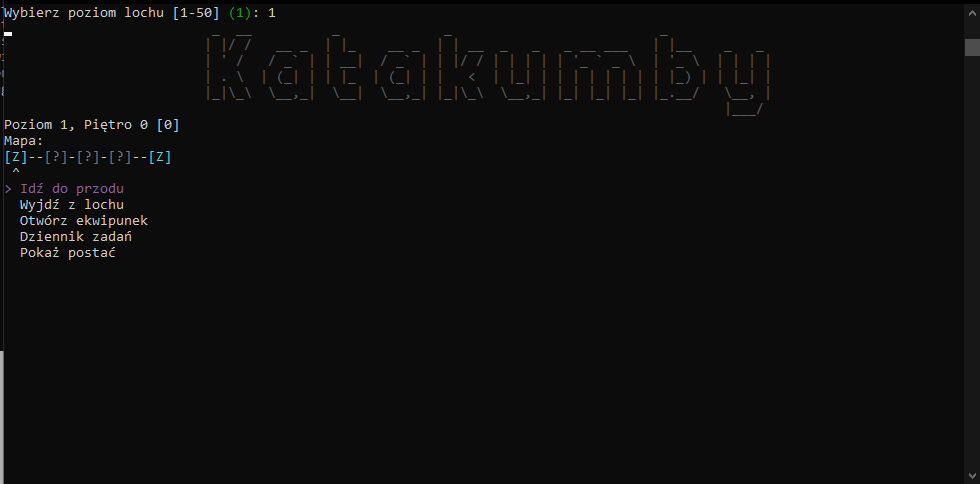
\includegraphics[width=0.8\textwidth]{figures/warstwa_uzytkowa/lochy_2.png}
                \caption{Lochy, widok mapy}
                \label{fig:dungeons_2}
            \end{figure}
        \item Po wejściu do lochu, pokazują się opcje poruszania się po lochu 
        (przód i tył - jeśli gracz znajduje się na granicy pięter, mogą się zmieniać w góra, dół, lub całkowite wyjście).
        Gracz może z tego poziomu także otworzyć ekwipunek lub dziennik zadań. Te opcje działają dokładnie tak samo jak w mieście.
        Na rysunkach 4.27 i 4.28 przedstawiono poruszanie się po lochu.
            \begin{figure}[H]
                \centering
                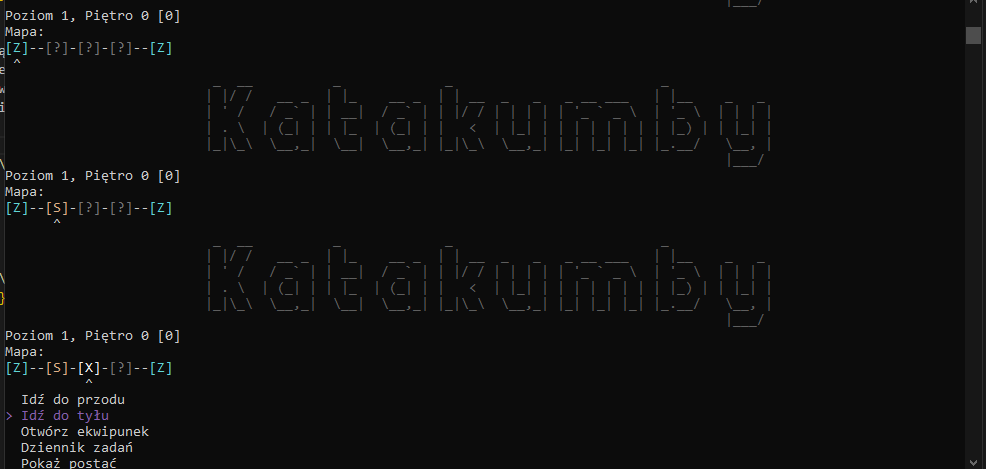
\includegraphics[width=0.8\textwidth]{figures/warstwa_uzytkowa/lochy_3.png}
                \caption{Lochy, poruszanie się w przód}
                \label{fig:dungeons_3}
            \end{figure}
            \begin{figure}[H]
                \centering
                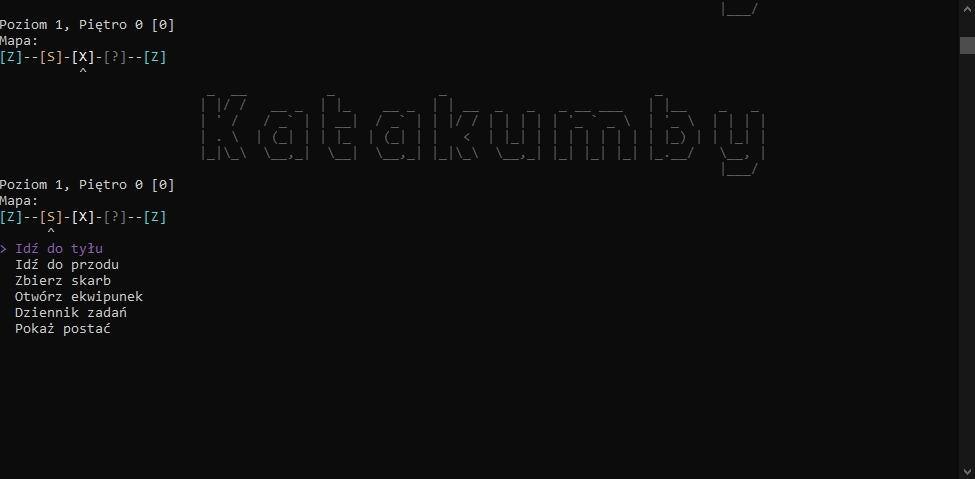
\includegraphics[width=0.8\textwidth]{figures/warstwa_uzytkowa/lochy_4.png}
                \caption{Lochy, poruszanie się w tył}
                \label{fig:dungeons_4}
            \end{figure}
        \item W lochach znajduje się wiele przedmiotów interaktowalnych: pułapki, walki, rośliny, skrzynki i ogniska. 
        W przypadku, gdy gracz napotka jeden z nich, może z nim interaktować poprzez odpowiednią opcję (np. `Zbierz skarb' widoczne na rysunku 4.28),
        lub interaktuje automatycznie po nadepnięciu na nie w przypadku walk i pułapek. Na rysunkach 4.29-4.31 pokazano interakcje z skrzynią, rośliną i ogniskiem.
            \begin{figure}[H]
                \centering
                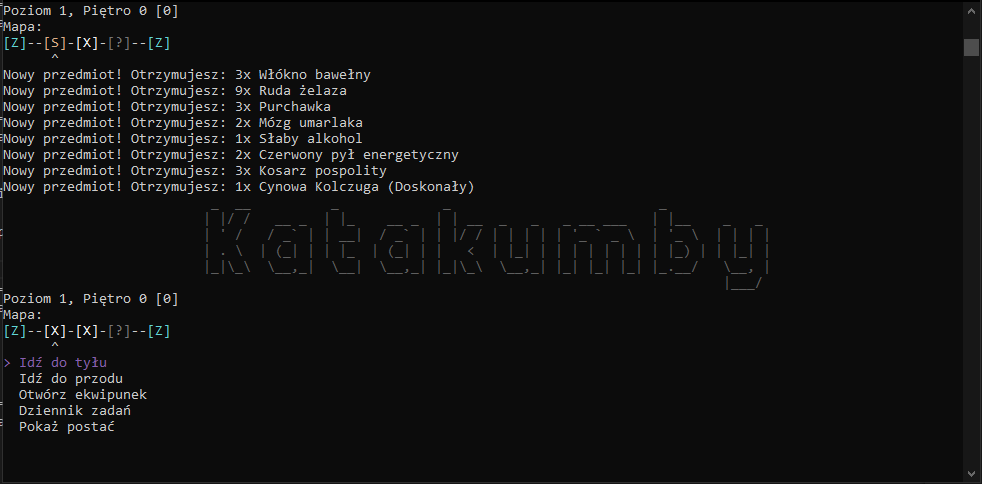
\includegraphics[width=0.8\textwidth]{figures/warstwa_uzytkowa/lochy_5.png}
                \caption{Lochy, otwieranie skrzyni}
                \label{fig:dungeons_5}
            \end{figure}
            \begin{figure}[H]
                \centering
                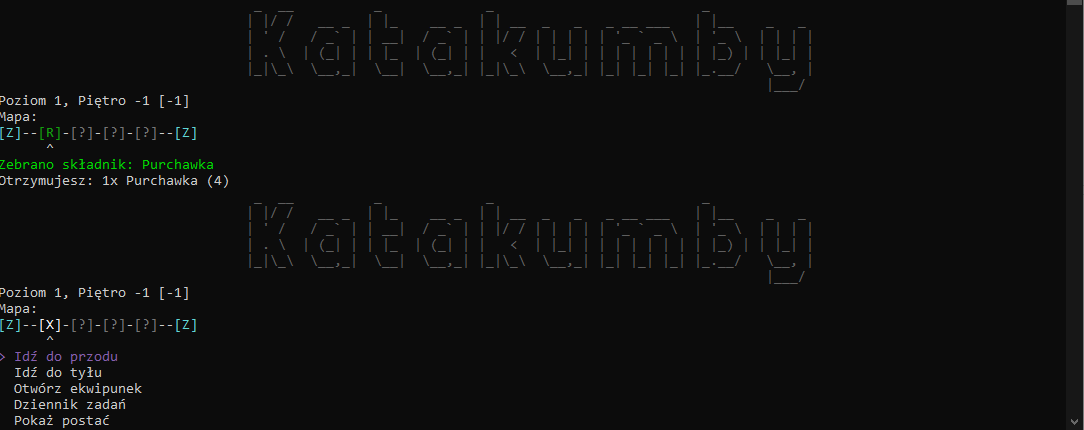
\includegraphics[width=0.8\textwidth]{figures/warstwa_uzytkowa/lochy_6.png}
                \caption{Lochy, zbieranie roślin}
                \label{fig:dungeons_6}
            \end{figure}
            \begin{figure}[H]
                \centering
                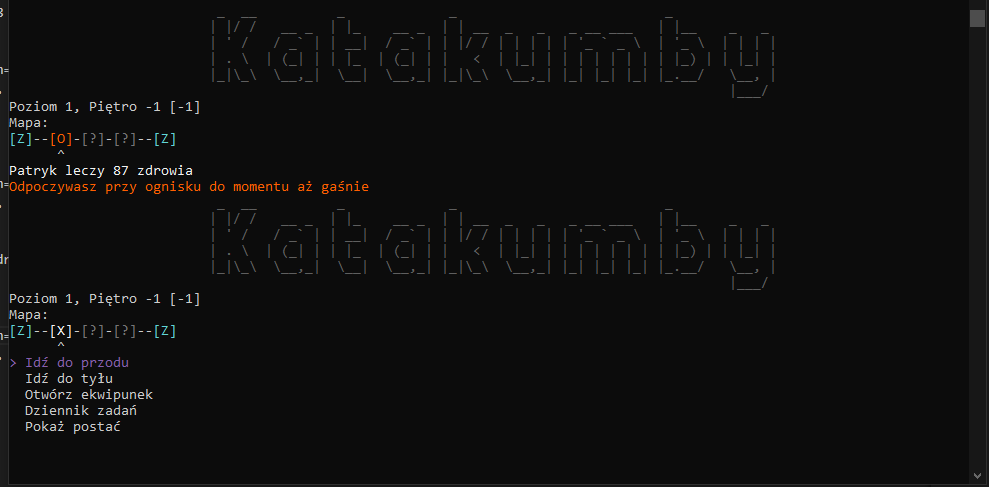
\includegraphics[width=0.8\textwidth]{figures/warstwa_uzytkowa/lochy_7.png}
                \caption{Lochy, odpoczywanie przy ognisku}
                \label{fig:dungeons_7}
            \end{figure}
\end{itemize}
\subsection{System walki}
\begin{itemize}
        \item Po napotkaniu walki w lochu, lub zasadzki podczas odpoczywania przy ognisku, rozpoczyna się ona automatycznie. 
        Użytkownik otrzymuje informację o przeciwniku i walka rozpoczyna się. Kolejność i częstość ruchów jest określana poprzez statystykę szybkości.
        W przykładzie gracz napotkuje przeciwnika `Upiór' i jest on szybszy, więc rusza się pierwszy. Gracz otrzymuje możliwość wykonania następnego ruchu.
        Gracz może dowolnie używać umiejętności, mikstur i wyświetlać informacje. Tura kończy się dopiero przy manualnym zakończeniu lub ucieczce.
        Na rysunku 4.32 przedstawiono rozpoczęcie walki
            \begin{figure}[H]
                \centering
                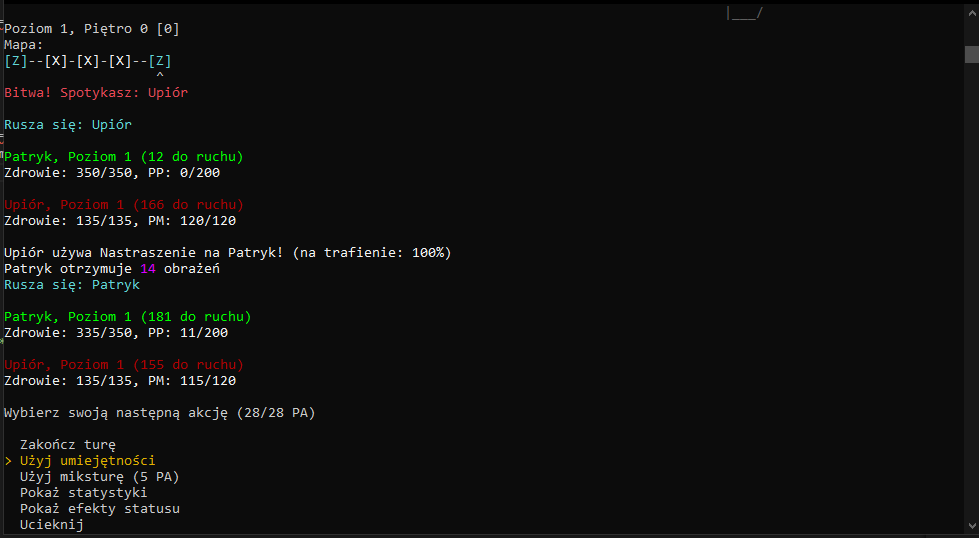
\includegraphics[width=0.8\textwidth]{figures/warstwa_uzytkowa/walka_1.png}
                \caption{System walki, rozpoczęcie walki}
                \label{fig:battles_1}
            \end{figure}
        \item Na rysunkach 4.33 i 4.34 przedstawiono użycie przez gracza umiejętności `Rzut Sztyletem'.
            \begin{figure}[H]
                \centering
                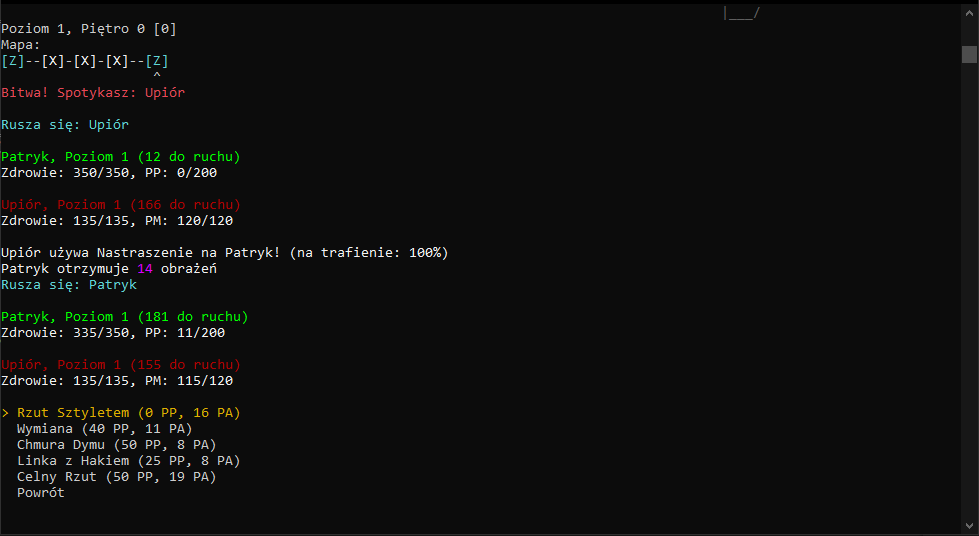
\includegraphics[width=0.8\textwidth]{figures/warstwa_uzytkowa/walka_2.png}
                \caption{System walki, wybór umiejętności}
                \label{fig:battles_2}
            \end{figure}
            \begin{figure}[H]
                \centering
                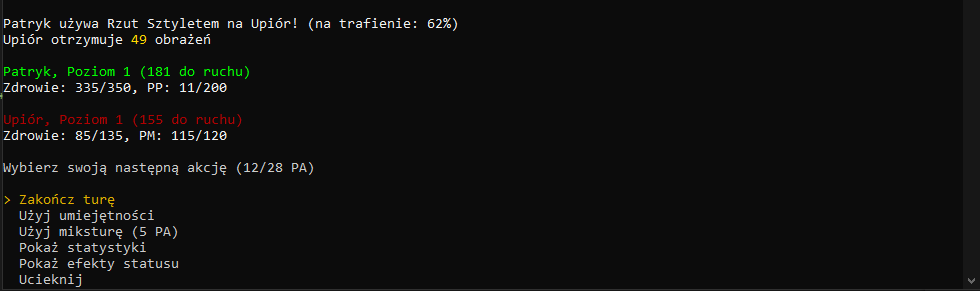
\includegraphics[width=0.8\textwidth]{figures/warstwa_uzytkowa/walka_3.png}
                \caption{System walki, użycie umiejętności}
                \label{fig:battles_3}
            \end{figure}
        \item Na rysunkach 4.35 i 4.36 przedstawiono nieudaną i udaną próbę ucieczki.
            \begin{figure}[H]
                \centering
                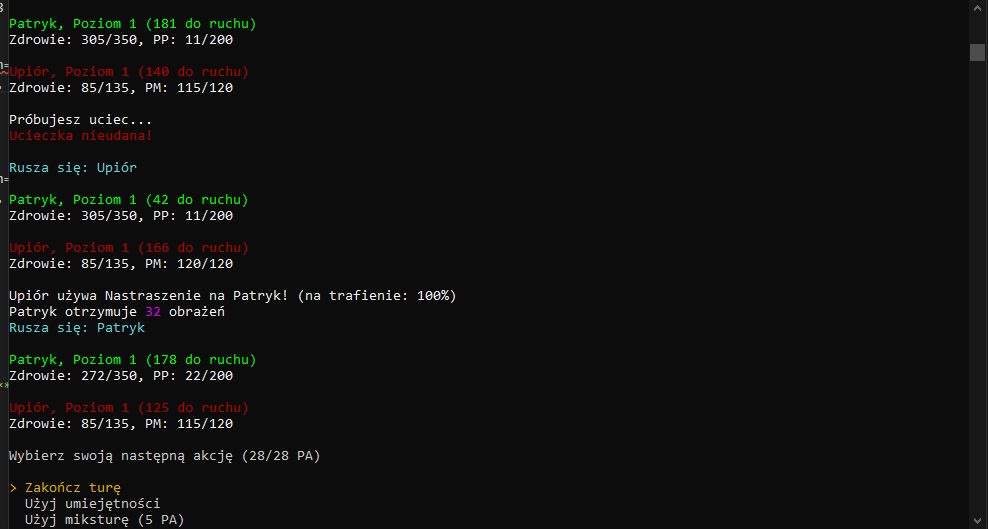
\includegraphics[width=0.8\textwidth]{figures/warstwa_uzytkowa/walka_4.png}
                \caption{System walki, nieudana ucieczka}
                \label{fig:battles_4}
            \end{figure}
            \begin{figure}[H]
                \centering
                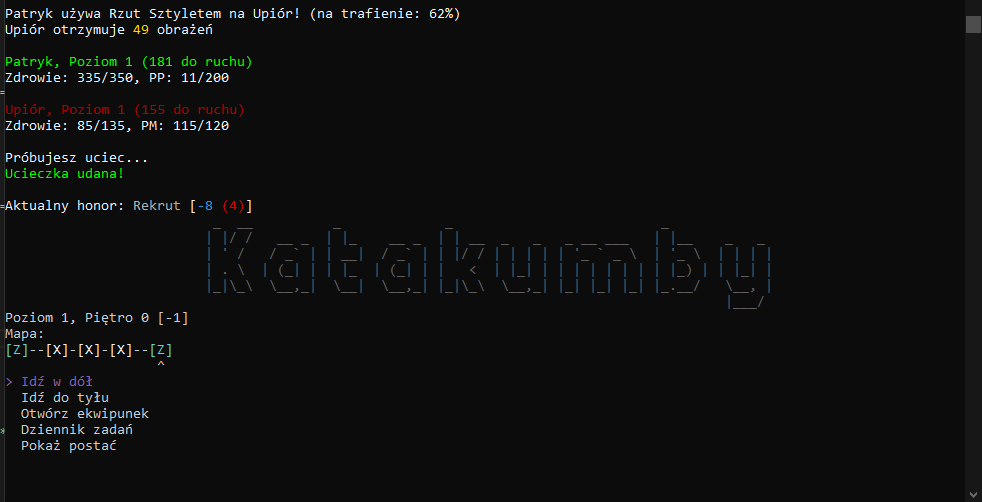
\includegraphics[width=0.8\textwidth]{figures/warstwa_uzytkowa/walka_5.png}
                \caption{System walki, udana ucieczka}
                \label{fig:battles_5}
            \end{figure}
        \item Walka kończy się, gdy zdrowie jednego z jej uczestników spadnie do 0. W przykładzie ukazanym na rysunku 4.37, gracz wygrywa
        i otrzymuje nagrody.
            \begin{figure}[H]
                \centering
                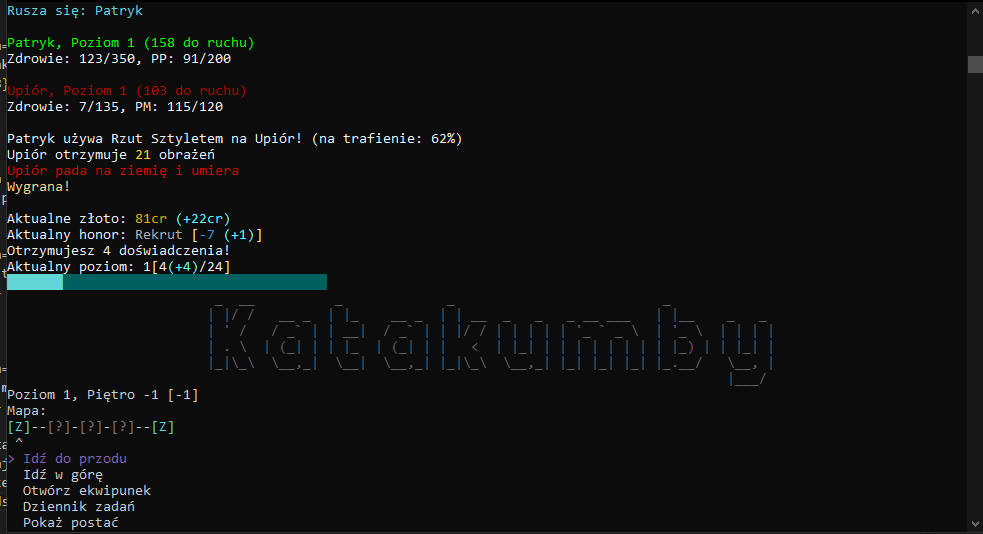
\includegraphics[width=0.8\textwidth]{figures/warstwa_uzytkowa/walka_6.png}
                \caption{System walki, nagrody za wygraną}
                \label{fig:battles_6}
            \end{figure}
\end{itemize}



% ********** Koniec rozdziału **********
